%%%%%%%%%%%%%%%%%%%%%%%%%%%%%%%%%%%%%%%%%
% Masters/Doctoral Thesis 
% LaTeX Template
% Version 2.5 (27/8/17)
%
% This template was downloaded from:
% http://www.LaTeXTemplates.com
%
% Version 2.x major modifications by:
% Vel (vel@latextemplates.com)
%
% This template is based on a template by:
% Steve Gunn (http://users.ecs.soton.ac.uk/srg/softwaretools/document/templates/)
% Sunil Patel (http://www.sunilpatel.co.uk/thesis-template/)
%
% Template license:
% CC BY-NC-SA 3.0 (http://creativecommons.org/licenses/by-nc-sa/3.0/)
%
%%%%%%%%%%%%%%%%%%%%%%%%%%%%%%%%%%%%%%%%%

%----------------------------------------------------------------------------------------
%	PACKAGES AND OTHER DOCUMENT CONFIGURATIONS
%----------------------------------------------------------------------------------------

\documentclass[
11pt, % The default document font size, options: 10pt, 11pt, 12pt
%oneside, % Two side (alternating margins) for binding by default, uncomment to switch to one side
english, % ngerman for German
singlespacing, % Single line spacing, alternatives: onehalfspacing or doublespacing
%draft, % Uncomment to enable draft mode (no pictures, no links, overfull hboxes indicated)
%nolistspacing, % If the document is onehalfspacing or doublespacing, uncomment this to set spacing in lists to single
%liststotoc, % Uncomment to add the list of figures/tables/etc to the table of contents
%toctotoc, % Uncomment to add the main table of contents to the table of contents
%parskip, % Uncomment to add space between paragraphs
%nohyperref, % Uncomment to not load the hyperref package
headsepline, % Uncomment to get a line under the header
%chapterinoneline, % Uncomment to place the chapter title next to the number on one line
%consistentlayout, % Uncomment to change the layout of the declaration, abstract and acknowledgements pages to match the default layout
]{MastersDoctoralThesis} % The class file specifying the document structure

\usepackage[utf8]{inputenc} % Required for inputting international characters
\usepackage[T1]{fontenc} % Output font encoding for international characters

\usepackage{mathpazo} % Use the Palatino font by default

\usepackage[backend=bibtex,style=authoryear,natbib=true]{biblatex} % Use the bibtex backend with the authoryear citation style (which resembles APA)
% numeric, alphabetic, authoryear, authortitle, verbose

\addbibresource{references.bib} % The filename of the bibliography

\usepackage[autostyle=true]{csquotes} % Required to generate language-dependent quotes in the bibliography

\usepackage{xcolor} % make colored boxes
\usepackage{color}
\usepackage{soul}

\setcounter{secnumdepth}{4} % makes subsubsection numbered
\setcounter{tocdepth}{4}

%----------------------------------------------------------------------------------------
%	MARGIN SETTINGS
%----------------------------------------------------------------------------------------

\geometry{
	paper=a4paper, % Change to letterpaper for US letter
	inner=2.5cm, % Inner margin
	outer=3.8cm, % Outer margin
	bindingoffset=.5cm, % Binding offset
	top=1.5cm, % Top margin
	bottom=1.5cm, % Bottom margin
	%showframe, % Uncomment to show how the type block is set on the page
}

%----------------------------------------------------------------------------------------
%	THESIS INFORMATION
%----------------------------------------------------------------------------------------

\thesistitle{A Nextflow Pipeline for the Predicion of Phenotype based on Metagenomc Data} % Your thesis title, this is used in the title and abstract, print it elsewhere with \ttitle
\supervisor{Dr. Sabrina Krakau} % Your supervisor's name, this is used in the title page, print it elsewhere with \supname
\examiner{Dr. Sven Nahnsen \\Prof. Dr. Nadine Ziemert} % Your examiner's name, this is not currently used anywhere in the template, print it elsewhere with \examname
\degree{Master of Science} % Your degree name, this is used in the title page and abstract, print it elsewhere with \degreename
\author{Matthias Marquardt} % Your name, this is used in the title page and abstract, print it elsewhere with \authorname
\addresses{} % Your address, this is not currently used anywhere in the template, print it elsewhere with \addressname

\subject{Bioinformatics} % Your subject area, this is not currently used anywhere in the template, print it elsewhere with \subjectname
\keywords{} % Keywords for your thesis, this is not currently used anywhere in the template, print it elsewhere with \keywordnames
\university{\href{http://www.university.com}{University of Tübingen}} % Your university's name and URL, this is used in the title page and abstract, print it elsewhere with \univname
\department{\href{http://department.university.com}{Informatik}} % Your department's name and URL, this is used in the title page and abstract, print it elsewhere with \deptname
\group{\href{http://researchgroup.university.com}{Quantitative Biology Center - QBiC}} % Your research group's name and URL, this is used in the title page, print it elsewhere with \groupname
\faculty{\href{http://faculty.university.com}{Mathematisch Naturwissenschaftliche Fakultät}} % Your faculty's name and URL, this is used in the title page and abstract, print it elsewhere with \facname

\AtBeginDocument{
\hypersetup{pdftitle=\ttitle} % Set the PDF's title to your title
\hypersetup{pdfauthor=\authorname} % Set the PDF's author to your name
\hypersetup{pdfkeywords=\keywordnames} % Set the PDF's keywords to your keywords
}

\begin{document}

\frontmatter % Use roman page numbering style (i, ii, iii, iv...) for the pre-content pages

\pagestyle{plain} % Default to the plain heading style until the thesis style is called for the body content

%----------------------------------------------------------------------------------------
%	TITLE PAGE
%----------------------------------------------------------------------------------------

\begin{titlepage}
\begin{center}

\vspace*{.06\textheight}
{\scshape\LARGE \univname\par}\vspace{1.5cm} % University name
\textsc{\Large Master Thesis}\\[0.5cm] % Thesis type

\HRule \\[0.4cm] % Horizontal line
{\huge \bfseries \ttitle\par}\vspace{0.4cm} % Thesis title
\HRule \\[1.5cm] % Horizontal line
 
\begin{minipage}[t]{0.4\textwidth}
\begin{flushleft} \large
\emph{Author:}\\
\authorname % Author name - remove the \href bracket to remove the link
\end{flushleft}
\end{minipage}
\begin{minipage}[t]{0.4\textwidth}
\begin{flushright} \large
\emph{Supervisor:} \\
\supname \\ % Supervisor name - remove the \href bracket to remove the link
\emph{Examiner:} \\
\examname  
\end{flushright}
\end{minipage}\\[3cm]
 
\vfill

\large \textit{A thesis submitted in fulfillment of the requirements\\ for the degree of \degreename}\\[0.3cm] % University requirement text
\textit{in the}\\[0.4cm]
\groupname\\\deptname\\[2cm] % Research group name and department name
 
\vfill

{\large \today}\\[4cm] % Date
%\includegraphics{Logo} % University/department logo - uncomment to place it
 
\vfill
\end{center}
\end{titlepage}

%----------------------------------------------------------------------------------------
%	DECLARATION PAGE
%----------------------------------------------------------------------------------------

\begin{declaration}
\addchaptertocentry{\authorshipname} % Add the declaration to the table of contents
\noindent I, \authorname, declare that this thesis titled, \enquote{\ttitle} and the work presented in it are my own. I confirm that:

\begin{itemize} 
\item This work was done wholly or mainly while in candidature for a research degree at this University.
\item Where any part of this thesis has previously been submitted for a degree or any other qualification at this University or any other institution, this has been clearly stated.
\item Where I have consulted the published work of others, this is always clearly attributed.
\item Where I have quoted from the work of others, the source is always given. With the exception of such quotations, this thesis is entirely my own work.
\item I have acknowledged all main sources of help.
\item Where the thesis is based on work done by myself jointly with others, I have made clear exactly what was done by others and what I have contributed myself.\\
\end{itemize}
 
\noindent Signed:\\
\rule[0.5em]{25em}{0.5pt} % This prints a line for the signature
 
\noindent Date:\\
\rule[0.5em]{25em}{0.5pt} % This prints a line to write the date
\end{declaration}

\cleardoublepage

%----------------------------------------------------------------------------------------
%	QUOTATION PAGE
%----------------------------------------------------------------------------------------

%\vspace*{0.2\textheight}
%
%\noindent\enquote{\itshape Thanks to my solid academic training, today I can write hundreds of words on virtually any topic without possessing a shred of information, which is how I got a good job in journalism.}\bigbreak
%
%\hfill Dave Barry

%----------------------------------------------------------------------------------------
%	ABSTRACT PAGE
%----------------------------------------------------------------------------------------

\begin{abstract}
\addchaptertocentry{\abstractname} % Add the abstract to the table of contents
The Thesis Abstract is written here (and usually kept to just this page). The page is kept centered vertically so can expand into the blank space above the title too\ldots
\end{abstract}

%----------------------------------------------------------------------------------------
%	ACKNOWLEDGEMENTS
%----------------------------------------------------------------------------------------

\begin{acknowledgements}
\addchaptertocentry{\acknowledgementname} % Add the acknowledgements to the table of contents
The acknowledgments and the people to thank go here, don't forget to include your project advisor\ldots
\end{acknowledgements}

%----------------------------------------------------------------------------------------
%	LIST OF CONTENTS/FIGURES/TABLES PAGES
%----------------------------------------------------------------------------------------

\tableofcontents % Prints the main table of contents

%\listoffigures % Prints the list of figures

%\listoftables % Prints the list of tables

%----------------------------------------------------------------------------------------
%	ABBREVIATIONS
%----------------------------------------------------------------------------------------

\begin{abbreviations}{ll} % Include a list of abbreviations (a table of two columns)

\textbf{LAH} & \textbf{L}ist \textbf{A}bbreviations \textbf{H}ere\\
\textbf{WSF} & \textbf{W}hat (it) \textbf{S}tands \textbf{F}or\\

\end{abbreviations}

%----------------------------------------------------------------------------------------
%	PHYSICAL CONSTANTS/OTHER DEFINITIONS
%----------------------------------------------------------------------------------------

%\begin{constants}{lr@{${}={}$}l} % The list of physical constants is a three column table

% The \SI{}{} command is provided by the siunitx package, see its documentation for instructions on how to use it

%Speed of Light & $c_{0}$ & \SI{2.99792458e8}{\meter\per\second} (exact)\\
%Constant Name & $Symbol$ & $Constant Value$ with units\\

%\end{constants}

%----------------------------------------------------------------------------------------
%	SYMBOLS
%----------------------------------------------------------------------------------------

%\begin{symbols}{lll} % Include a list of Symbols (a three column table)
%
%$a$ & distance & \si{\meter} \\
%$P$ & power & \si{\watt} (\si{\joule\per\second}) \\
%%Symbol & Name & Unit \\
%
%\addlinespace % Gap to separate the Roman symbols from the Greek
%
%$\omega$ & angular frequency & \si{\radian} \\
%
%\end{symbols}

%----------------------------------------------------------------------------------------
%	DEDICATION
%----------------------------------------------------------------------------------------

%\dedicatory{For/Dedicated to/To my\ldots} 

%----------------------------------------------------------------------------------------
%	THESIS CONTENT - CHAPTERS
%----------------------------------------------------------------------------------------

\mainmatter % Begin numeric (1,2,3...) page numbering

\pagestyle{thesis} % Return the page headers back to the "thesis" style

% Include the chapters of the thesis as separate files from the Chapters folder
% Uncomment the lines as you write the chapters


\chapter{Introduction} % Main chapter title

\label{introduction} % Change X to a consecutive number; for referencing this chapter elsewhere, use \ref{ChapterX}

%----------------------------------------------------------------------------------------

% Define some commands to keep the formatting separated from the content 
\newcommand{\keyword}[1]{\textbf{#1}}
\newcommand{\tabhead}[1]{\textbf{#1}}
%\newcommand{\code}[1]{\colorbox{lightgray}{\texttt{#1}}}
\newcommand{\code}[1]{{\sethlcolor{lightgray}\hl{\texttt{#1}}}}
\newcommand{\file}[1]{\texttt{\bfseries#1}}
\newcommand{\option}[1]{\texttt{\itshape#1}}

%----------------------------------------------------------------------------------------


\section{Metagenomics}

Since the human genome project, where in a massive collaborative effort the first human genome has been sequenced and assembled, Next generation sequencing (NGS) methods have taken over. 
NGS methods like sequencing by synthesis, which is used in Illumina sequencing machines, enabled the creation of huge amounts of data. 
% wgs, shotgun vs 16s

The general importance of metagenomics has just become clear in the recent years. 
% examples needed
Certain illnesses are not only determined by genome and lifestyle but also by the microbiome composition of affected body parts. % which ones? 

For example some species and strains are implicated in causing inflammatory bowel disease (IBD) % more specific



\section{Machine Learning and Reproducibility}

Recent advances in computing power enabled the extensive use of Machine Learning (ML) algorithms. 
Frameworks like \keyword{scikit-learn} have become better and popular \citep{scikit}.

Algorithms like Support Vector Machines (SVM), Random Forest (RF) and Gradient-Boosted Trees (XG-Boost) have been successfully used to predict illnesses based on metagenomic data before. These studies lack a focus on reproducibility and do not have best practices in mind.

\citep{xgboost}
% FOSS important for reproducibility

\section{Thesis Objective}
Exploration of publicly available datasets 

Create a pipeline which makes conducting Machine Learning experiments on metagenomic data for phenotype prediction reproducible. The pipeline should be designed following best practices so potential users do not have to focus on this.
% taxonomic profiler

\chapter{Theoretical Background} 

\label{theory} 


% should contain
% metagenomics/microbiome
% ML -> RF, XGB, SVM
% Workflowmanager for reproducibility -> Nextflow
% wich of these aproaches has been used before? -> metapheno, metaml

\section{Metagenomics}

Real world data is ugly. It contains a lot of noise. Microbiome reads can be contaminated with host DNA and with adapters from sequencing. In order to clean up the data preprocessing has to be performed. 

% single end, pair end where to put it exactly??


	\subsection{File formats}
Sequencing is the technique of translating the succession of nucleotides into a string. In order to save this digitized DNA information two standard file formats have prevailed: FASTA and FASTQ. 

FASTA is a relatively simple format. It uses two lines per sequence. A read begins with the character \code{>} followed by the name of the read (unique identifier), a newline character \code{\textbackslash n} and then the sequence of the read which is usually ended with a newline character, then this can be repeated in case of multiple reads. The DNA sequence usually is encoded with the letters A,C,T and G (can also be lower case) for the bases Adenine, Cytosine, Thymine and Guanine.
% maybe to detailed
The general file suffix is .fasta. The FASTA file format can also represent amino acid so in order to distinguish the two the recommended suffixes are .faa for amino acids and .fna for nucleotides.
FASTQ encodes the sequence as well as its corresponding quality score. Per sequence 4 lines are used. 
The first line begins with the \code{@} character followed by the sequence identifier (systematic use with Illumina, encodes machine used, lane, etc).
The second line contains the raw sequence.
The third line starts with the \code{+} character optionally followed by the same sequence identifier as in used the first line.
The fouth line contains the encoded quality scores corresponding to the second line, therefore it has to have the same number of symbols than the sequence itself.
% a rough explanation of it
The quality scores are encoded using the order of ASCII (American Standard of Code Information Interchange) characters. Starting with the 33rd ASCII character \code{!} representing lowest quality the original encoding goes up to character 126 \code{\textasciitilde} as the highest encoded quality score possible. Today the most widely used encoding is called Pred+33 (i.e. used by Illumina). It only encodes up to character 74 \code{J} as highest quality score.

	\subsection{Preprocessing}
The quality information in a FASTQ file can be leveraged to only keep part of a sequence which are reliable. If the quality score falls below a set threshold reads can be cut so that only meaningful data is used.

When using microbiome reads there is always the possibility of reads still containing host DNA. In order to clean up all the reads are compared to a library of the host genome and matches are removed.
% phix removal ?, explanation right, tmi?
In Illumina sequencing the PhiX library can used as an internal standard. It is a library of well maintained and characterized phage genomes. They are not always removed correctly when using publicly available datasets. In order to ensure no contamination of the reads they can be removed by comparing to the known genome. 

	\subsection{Taxonomic profiling}
After preprocessing the more interesting questions can be asked. What kind of microbes are in the sample?

% taxonomic tree, insert graphics, 
% explain clades
In order to classify groups of organisms and display their hierarchy biologists use the taxonomic rank. The main taxonomic ranks from generic to specific are: domain, kingdom, phylum, class, order, family, genus and species. For metagenomics the genus and species level are used the most. 
In 2020 3,433 (± 115) bacterial genus names were accepted \citep{genus}.
Strains are subtypes of species which is extremely useful for a even more fine grained resolution of the sample composition.
% genus size, species size

Taxonomic profilers use preprocessed reads to estimate the relative composition of microbes in the probe.
There are different kinds of taxonomic profilers, MetaPhlan3 and kraken2 are two widely used examples. 

% make mpa and kraken subsubsections?
%\subsubsection{MetaPhlAn3}
% way to unspecific
MetaPhlAn3 (\textbf{Meta}genomic \textbf{Ph}y\textbf{l}ogenetic \textbf{An}alysis) is the third iteration of a taxonomic profiling software from the Segata Lab. It is reference based, which means it uses the coverage of clade specific marker genes in a sample to estimate the taxonomic composition.
The marker genes are chosen such that all strains in a clade posses them while other clades contain no orthologes which are close enough to match as well. \citep{mpa3}
MetaPhlAn3 contains 1.1M marker genes from around 13.5 k species.

%\subsubsection{kraken2}
% way to unspecific
kraken2 is reference based and uses a huge database to compare the sample to. From the query sample k-mers are extracted and matches in the database to assign the Lowest Common Ancestor (LCA). This information is used to estimate the relative species composition of the sample. \citep{kraken2}



\section{Machine Learning}
In order to get meaningful results with ML problems have to be framed correctly. The goal of a study determines the methods and algorithms that have to be used. 
What is the objective has to be one of the first questions asked. Is it sufficient to put samples in two or more distinct categories or are the samples differing in severity? The first would be a classification problem while the second case would be a regression problem.   
% mention clustering?
Another important distinction of ML algorithms is weather they are using supervised or unsupervised learning. This is dependent on the data as supervised algorithms need clearly labeled training data. The training data is used to optimize the performance so that unseen data can be categorized correctly by the algorithm. Unsupervised learning uses untagged data where algorithms try to find underlying patterns.

A pitfall to be aware of when using supervised learning problems is overfitting. The internal model used is to complex. This means that the algorithm has learned specifics of the training data and it is not generalizing well. It then has problems predicting new and unseen data. 

Cross-validation is a technique that can be used to asses the generalization of an given algorithm. It can thus be used to prevent overfitting. 
Data is split in training and validation set, this can be done multiple times following certain schemes.
% leave-one-out, k-fold, nested

Feature selection can also be used to prevent overfitting. It can shorten training times and help to avoid the curse of dimensionality.
% how does it work?

% Hyperparamters and tuning
Implementations of ML algorithms usually need more input than the training data, they have so called hyperparameters which need to be adjusted in order to optimize the results. Each algorithm has its own set of hyperparameters and the tuning of them is a very important but time intensive step.

In recent years a wide range of ML algorithms has been developed. The following sections describe some of the most widely used algorithms for supervised classification.

	\subsection{Support Vector Machines}
Suppose a dataset with two classes. In order to classify the data points a SVM will try to construct a hyperplane which separates the data points of those two classes. 
There can be many ways that a hyperplane separates the data so a reasonable choice is to maximize the margin, which is the distance between the data points and the hyperplane. % a bit to vague, maybe?
Nonlinear data can be classified with a SVM as well. To enable this the kernel trick is needed. The feature space is transformed to a higher dimension which makes it possible to fit a linear hyperplane. For this polynomial or Gaussian radial basis function kernels can be used.

% add formal mathmatical definitions!

% what are the hyperparameters
 
	\subsection{Random Forests}
Random forests are a ensemble learning method taking multiple decision trees and averaging their results.

%Decision tree
%observation represented in branches (features), target value in leaves (classification)

Individual decision trees tend to overfit the training data. RF learning averages over multiple deep trees trained from different parts of data set. This reduces variance, but leads to a small increase in bias and a marginal decreased interpretability compared to individual decision trees. Generally the interpretability is a wished feature and it is still given through the variable importance.

%bootstrap aggregating (bagging)
%bagging decreases variance, without increasing the bias

% what are the hyperparameters

	\subsection{Gradient Boosted Trees}
Ensemble method
boosting: multiple weak learners into a strong one
iteratively learning weak learners, adding to the strong learner after adding data weights are readjusted (re-weighing) misclassified input gets higher weight so future learners focus more on them
weak learners are added using a gradient descent optimization algorithm


% what are the hyperparameters


	\subsection{Evaluation of Machine Learning algorithms}
Different metrics have been proposed and are being used to optimize and evaluate the effectiveness of ML algorithms. Which of these are best is not clear. There are no standards yet as the importance of respective advantages and disadvantages are still being debated. It is better to use many metrics and not completely rely on one.

% roc
%(balanced) accuracy
% precision
% recall
% f1-score
% mcc




\section{Workflowmanagers and Reproducibility}
In order to generate meaningful results preprocessing, profiling, training and prediction have to be brought together. For this different scripts have to be executed sequentially. For one dataset this is fairly straight forward. But for multiple datasets it can get repetitive and error prone as the same scripts have to be executed over and over with slightly different parameters.  
Workflow management frameworks can be used to build pipelines which automate the execution of scripts and thus help to avoid time costly errors. In combination with containers they can enable experiments being conducted independent of the hardware used making them portable. 
Using a workflowmanager is a big step towards reproducibility as the execution of a pipeline with the same parameters should yield the same result. This only holds if there inherent randomness in the pipeline. For machine learning this means that only CPU powered learning can be truly reproducible and only if all seeds are set to fixed values.
% sklearn for example
% mention GPUs?

A lot of workflow management frameworks have been developed and new ones are being published continuously. Snakemake and Nextflow are among the most popular as they have strong community support.
Both are Command Line Interface (CLI) programs and support the usage of containers as well as version control systems like git. They use their own Domain Specific Language (DSL) as extensions of the underlying programming language, Groovy for Nextflow and Python for Snakemake.

Snakemake executes operations based on a directed acyclic graph (DAG). Each step is represented by rules which describe the handling of input and output files. The DAG is derived inferred from the set of all rules  \citep{snakemake}. 

In the Nextflow dataflow model operations are executed in their own isolated process. The output of a process then is streamed through a channel into processes dependent on the previous output. This enables parallel execution of tasks and a high scalability \citep{nextflow}.
Around Nextflow a vivid community has developed with nf-core. Best practices pipelines for a wide range of use cases have been developed and are being curated. They are easily accessible and have extensive documentation. Questions can be asked in the very active Slack workspace. A starter template helps developers following best practices \citep{nfcore}.

\section{Previous work}
strengths and weaknesses 
reasoning and importance of my work, placement in field of research -> no pipeline yet, stuff is not reproducible 
% maybe better in intro/objective ?




\chapter{Experimental Setup} 

\label{experimental_setup} 
% maybe name it considerations of pipeline design or something like this

% should contain
% pipeline architecture
% genus/strain/species
% strain+species

\section{Design considerations}
One of the main goals of this master thesis was to design a Nextflow pipeline performing reproducible machine learning. 
There are some research questions which influence the design choices taken.
With MetaPhlAn3 and kraken2 two different taxonomic profilers have been implemented. Other taxonomic profilers could be added in the future as well. This flexibility enables potential users to chose the best fitting profiler for their task or experiment if unsure.

Another important aspect is the taxonomic level on which the ML algorithm is learning its patterns. Depending on the illness genus, species, strain or a combination of species and strain is the more important. The user can decide which of these levels to looked at, or even use all of the above in order to learn which the most distinguishing levels for a certain illness are.

There are different ML algorithms implemented. The user can chose between SVM, RF, XG-Boost and L2-Linear Regression or take a multiple of them. 
% mention L2?
A feature selection can be indicated with its corresponding threshold value. The metric on which the algorithm optimizes is customizable. 
% can be chosen? MCC, balanced accuracy as sensible defaults


\section{Pipeline architecture}


\begin{figure}
	\centering
	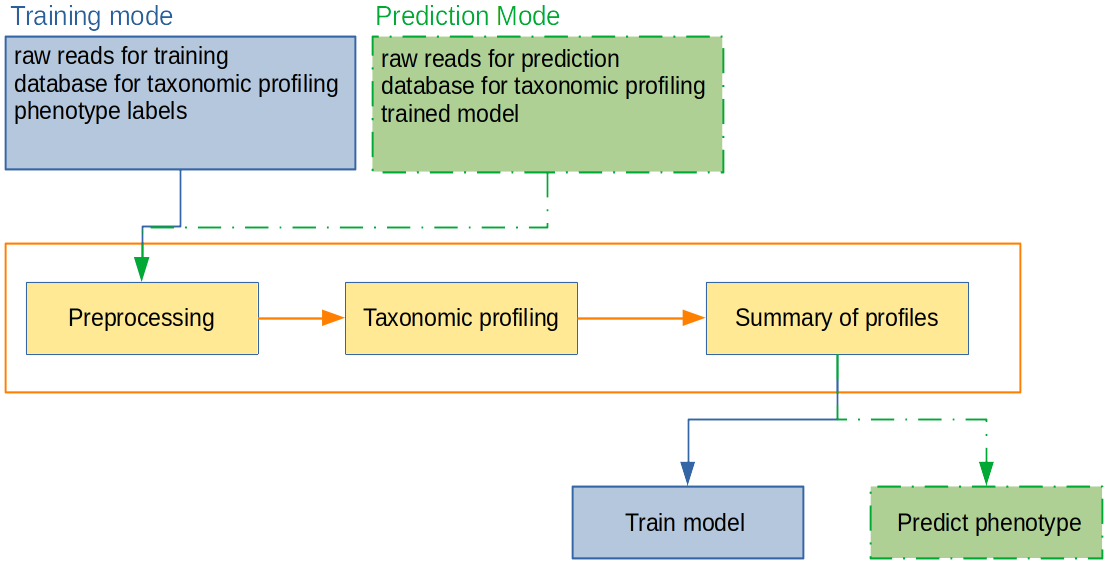
\includegraphics[width=0.9\textwidth]{Figures/pipeline_schemata_rev}
	%\decoRule
	\caption{Schema of the pipeline architecture. Train mode is blue colored, predict mode is green and the shared components are colored yellow.}
	\label{fig:schema}
\end{figure}


The Nextflow pipeline developed within this master thesis takes metagenomic data as input and trains a phenotype prediction algorithm with this information. It then can be used on unseen data for prediction.
Figure \ref{fig:schema} shows a schematic overview of the underlying architecture. 
% Train / predict mode
The pipeline has two distinct modes: training and prediction. Both modes share a common processing steps. Reads are trimmed based on their quality, host contamination is removed, taxonomic profiling is performed and summarized.

% how is the pipeline executed, example with paramters and flags

\subsection{Preprocessing}
Quality based trimming is performed with fastp \citep{fastp}. The 3'-end and the 5'-end are trimmed if the quality score in a sliding window falls below a preset threshold. Fastp is executed with these parameters:
\\
\code{fastp -q mean\_quality -{}-cut\_by\_quality5 -{}-cut\_by\_quality3 -{}-cut\_mean\_quality trimming\_quality}
\\
The quality score in the sliding window is set with the pipeline parameters \code{trimming\_quality} and \code{mean\_quality} which have a default value of 15.\\
% -M, --cut_mean_quality               the mean quality requirement option shared by cut_front, cut_tail or cut_sliding. Range: 1~36 default: 20 (Q20) (int [=20])
% -q, --qualified_quality_phred      the quality value that a base is qualified. Default 15 means phred quality >=Q15 is qualified. (int [=15])

% process in nextflow pipeline, should i mention it?

If host DNA is present it can be removed with bowtie2 \citep{bowtie2}.
To achieve this a fasta file of the host has to be provided. bowtie2 then finds and removes matches of the host DNA in the samples.

\subsection{Taxonomic profiling}
% mpa, kraken
By default both MetaPhlAn3 and kraken2 are used for taxonomic profiling. 
\code{-{}-skip\_metaphlan} and \code{-{}-skip\_kraken2} can be specified on pipeline execution when just one profiler is wished.
The databases are downloaded and configured automatically. If they are already present on the executing system their path can be specified with \code{-{}-kraken2\_db "\$PATH"} or \code{-{}-metaphlan\_db "\$PATH"} where \code{"\$PATH"} is a placeholder for the database path on the executing machine.

% execution with default parameters, can be changed

For each taxonomic profiler a summary table of all sample profiles is created with a custom python script using the pandas framework \citep{pandas}.

\subsection{Training mode}

% feature selection here

% data splitting for cv
% python script using scikit-learn
Figure \ref{fig:trainsplit} shows the data splitting scheme which is used during training mode. A custom python script uses the previously created summary table of taxonomic profiles to train the specified classifiers. All of the classifiers are implemented either in the scikit-learn or XGBoost packages.

% report of runtime and mean evaluation values
Finally mean values of ROC, (Balanced) Accuracy, Precision, Recall, F1-Score and MCC are reported together with the runtime. The trained classifiers are pickled and saved so that they can be used in the prediction mode. 

\begin{figure}
	\centering
	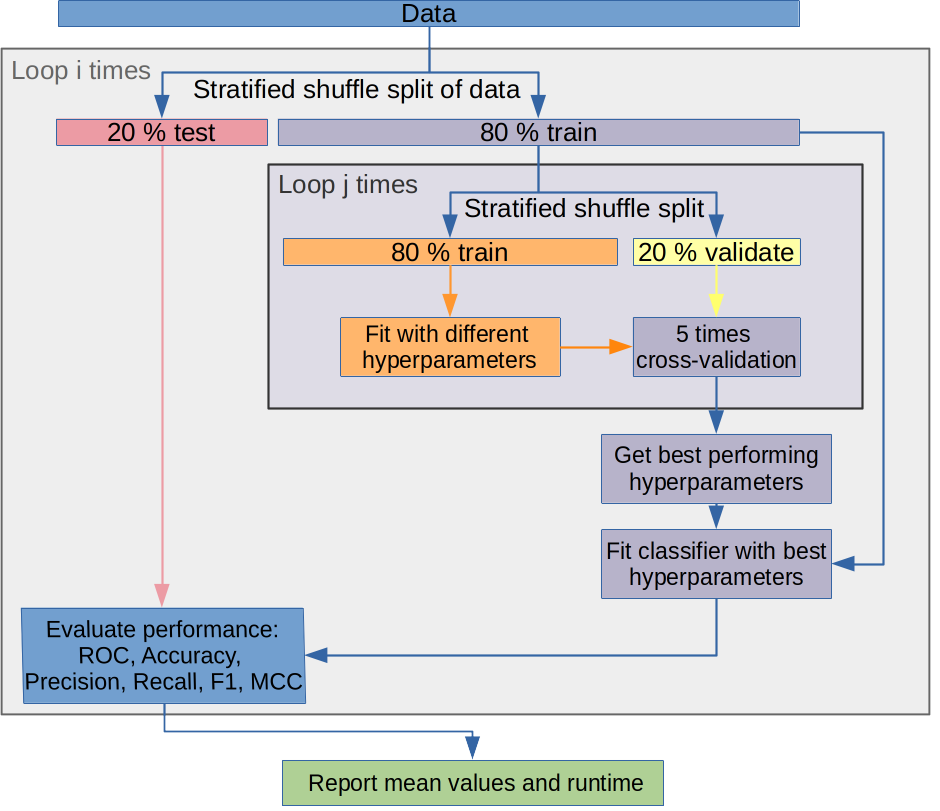
\includegraphics[width=0.9\textwidth]{Figures/ml_evaluation_datasplit_rev}
	%\decoRule
	\caption{Data splitting schema for testing and training. A stratified shuffle split is performed i-times on all of the data, respectively putting 20\% into the testing and 80\% in training set. Each training set is split j-times into 20\% validation and 80\% hyperparameter-training set. Five times cross-validation is used with this validation and training set to get the best performing hyperparameters. The performance then is evaluated i-times on the original test/train splits. Mean values and runtime are reported.}
	\label{fig:trainsplit}
\end{figure}


\subsection{Prediction mode}
% what class are the samples belonging to
For prediction mode one or more pretrained classifiers and the samples have to be provided. The same preprocessing and taxonomic profiling which has been used in training mode is performed on the samples. For the classification a python script uses the summary table of the taxonomic profiles and the classifiers yielding a prediction. 


% moved from results
\section{Datasets}

%which ones have been used, selection process, number of samples etc
There are several benchmark datasets which have been used for phenotype prediction.  Liver cirrhosis has yielded very good results before. Obesity is a hard case as researchers have struggled to get good performing predictions. Inflammatory Bowel Disease (IBD) is used as a smaller and imbalanced dataset yielding promising results. The number of samples and the size of the datasets is shown in table \ref{tab:datasets}. 


\begin{table}[]
	\centering
	\caption{Cases and sample size of considered datasets. Their size is given in Terabasepairs.}
	\label{tab:datasets}
	\begin{tabular}{lllll}
		\hline
		& Disease Cases & Healthy Cases & Total Samples & Size {[}Tbp{]} \\ \hline
		Liver Cirrhosis & 123     & 114    & 237   & 1.2            \\
		Obesity         & 169     & 123    & 292   & 1.6            \\
		IBD             & 25      & 99     & 124   & 0.39           \\ \hline
	\end{tabular}
\end{table}
 
\chapter{Results and Data Analysis}
% 'Results and Discussion' better?
\label{results} 


% should contain:
% runtime measurements
% genus/strain/species
% strain+species
% ML scoring function and feature selection


\section{ML evaluation}
% maybe overview table?

\section{Algorithm choice}
% which algo is best? depends

\section{Performance of taxonomic profilers}
% where is kraken better? mpa good performance overall

\section{Influence of taxonomic level}
% depends on illness, strain+species appears to be good

\section{Feature selection}
% reduces runtime, not much else here

\section{Runtime measurements}
% need to figure this out --> do measurements!!!





% Chapter Template

\chapter{Conclusion and Outlook} % Main chapter title

\label{ChapterX} % Change X to a consecutive number; for referencing this chapter elsewhere, use \ref{ChapterX}

% what did work, what did not?
% result is a functional pipeline, which can be extended, is reproducible, portable and stable

\section{Possible Extensions}

bracken
mlf-core
dsl2
% if sequencing grows exponentialy, sql for data summary 
%\include{Chapters/06_Conclusion} 

%----------------------------------------------------------------------------------------
%	THESIS CONTENT - APPENDICES
%----------------------------------------------------------------------------------------

\appendix % Cue to tell LaTeX that the following "chapters" are Appendices

% Include the appendices of the thesis as separate files from the Appendices folder
% Uncomment the lines as you write the Appendices

%% Appendix A

\chapter{Frequently Asked Questions} % Main appendix title

\label{AppendixA} % For referencing this appendix elsewhere, use \ref{AppendixA}

\section{How do I change the colors of links?}

The color of links can be changed to your liking using:

{\small\verb!\hypersetup{urlcolor=red}!}, or

{\small\verb!\hypersetup{citecolor=green}!}, or

{\small\verb!\hypersetup{allcolor=blue}!}.

\noindent If you want to completely hide the links, you can use:

{\small\verb!\hypersetup{allcolors=.}!}, or even better: 

{\small\verb!\hypersetup{hidelinks}!}.

\noindent If you want to have obvious links in the PDF but not the printed text, use:

{\small\verb!\hypersetup{colorlinks=false}!}.

%\include{Appendices/AppendixB}
%\include{Appendices/AppendixC}

%----------------------------------------------------------------------------------------
%	BIBLIOGRAPHY
%----------------------------------------------------------------------------------------

\printbibliography[heading=bibintoc]

%----------------------------------------------------------------------------------------

\end{document}  
